\section{Design}
This chapter describes the general design of Tsukiji.
Motivations for the choices in our design will be discussed.
For more detailed issues during the process of implementation, see section \ref{implementation}.

\subsection{Architecture}
Tsukiji consists of two main modules (orderbook and trader), a cryptography module, and several smaller utility modules.
This is depicted in figure \ref{modulesfig}.
There are several third-party libraries Tsukiji depends on.
The important ones are described later on in section \ref{dependencies}.

The trader module consists mainly of the Trader class.
Its main purpose is to communicate with other remote Traders.
The Trader class is a subclass of the DatagramProtocol class provided by the Twisted library \cite{twisted}.
This means the Trader class implements the UDP protocol.
The UDP protocol is the transport protocol used to connect with other traders.
For more information on the application protocol used, see section \ref{protocol}.

The orderbook module has three main functionalities: 1. message creation for the application protocol and 2. managing the state of the orderbook itself and 3. matching bids and asks.
The message creation is used in combination with the trader module.
These are the messages that are passed around between peers.
Managing the state of the orderbook is an important task.
The orderbook keeps track of what offers come in, what offers are expired, or what trades have been made.
Finally, the matching algorithm is a simple yet effective algorithm.
For every incoming offer, the algorithm checks whether the trader has an offer that matches the incoming one.
It tries to match favourable trades against any incoming offers.
These functionalities are closely related, e.g. matching an ask with a bid produces a trade message, whereafter the orderbook is updated.

An example of a function in the first category is the function \texttt{create\_ask(price, quantity, timeout)}.
This function creates an 'ask' message, with a given price, quantity, and timeout.
An example of a function in the third category is the function \texttt{match\_bid(bid)}.
Given a bid as input, check if there are compatible asks from yourself and output the most favourable one.
The second category has few functions specifically created for this task.
Rather, it is managed mostly by side-effects from other functions.
For more detail, it is best to look at the code itself and its accompanying comments.

The cryptography module contains everything related to actions with public-key cryptography.
At the moment, it mostly functions as a wrapper around the PyCrypto library, for easier use within Tsukiji.
More on this can be read in section \ref{sprint1:identifiers}.

\begin{figure}
  \centering
  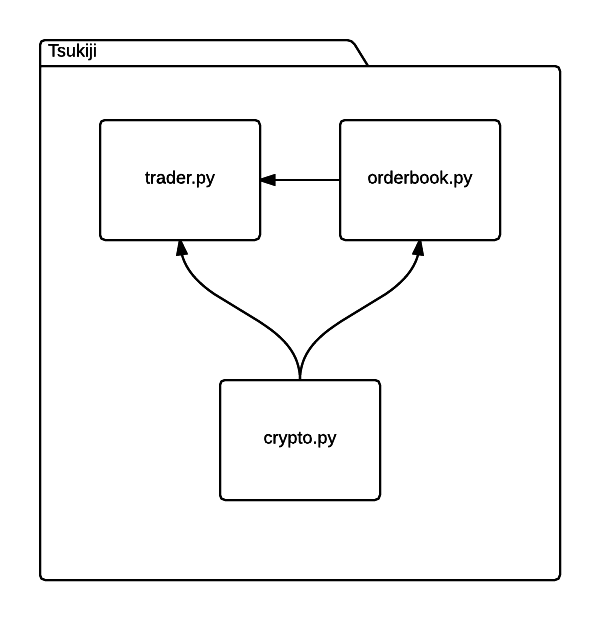
\includegraphics[width=\textwidth]{modules}
  \caption{A diagram with all of Tsukiji's modules}
  \label{modulesfig}
\end{figure}

\subsubsection{Dependencies}
\label{dependencies}
Tsukiji has two main dependencies: Twisted\cite{twisted} and PyCrypto\cite{pycrypto}.
Twisted is an open-source networking library.
It enjoys wide-spread use in the python world.
It has served Tsukiji particularly well with its implementation of the UDP protocol.
For more information, see section \ref{sprint2:twisted}.

% PyCrypto
PyCrypto is a cryptography toolkit for python.
It comes with many functions related to cryptography, but we are mostly interested in functions related to public-key cryptography.
Each trader has a public/private key pair.
A trader's public key acts as their identifier.
For more information, see section \ref{sprint1:identifiers}.

\subsection{Trade Protocol}
\label{protocol}

Tsukiji uses a custom application protocol to communicate between peers.
Traders communicate to each other with messages encoded as JSON objects.
The choice for JSON objects was made because it has a near-equivalent data type in python called a dictionary.
It is also a human-readable format.
Every message has the following additional attributes:
\begin{myitemize}
\item id: Public key of the trader sending the message.
\item message-id: Incremental counter unique across all messages with the same id.
\item timestamp: Time of creation of this message.
\item type: The type of message.
\end{myitemize}

There are 7 message types in total: ask, bid, trade, confirm, cancel, greeting, and greeting\_response. Each type of message is used in a different scenario and holds different attributes. In the following sections, these scenario's are laid out.

\subsubsection{Placing an offer}
In order to place an ask or bid, a message is sent where the type is 'ask' or 'bid' accordingly.
These types of messages have the following additional attributes:
\begin{myitemize}
\item price: The price per single unit.
\item quantity: The amount of items requested to trade.
\item timeout: The time of expiration for this offer.
\end{myitemize}

This type of message is typically sent to the entire network.

\subsubsection{Requesting a trade}
When a trader sees an offer they are interested in, they might respond to such an offer with a trade message.
The type of this message is 'trade'.
This type of message has the following additional attributes:

\begin{myitemize}
\item recipient: The id of the trader who created the offer.
\item quantity: The quantity requested to be traded.
\item trade-id: The message-id of the original offer.
\end{myitemize}

The combination of recipient and trade-id is used to uniquely identify the specific offer for which the trade is requested.
The quantity field may be equal to or less than the quantity stated in the original offer.
Perhaps a trader is interested in an offer, but only can or needs to trade a certain amount that is less than this.

\subsubsection{Accepting a trade}

When a trade request arrives, a trader can either accept or cancel such a request.
In the event that the trader accepts the trade request, they send a confirm message back.
The type of this message is 'confirm'.
This type of message has the following additional attributes:

\begin{myitemize}
\item trade-id: the message-id of the original offer.
\end{myitemize}

This time, there's no need to add a recipient attribute because the combination of the 'id' and 'trade-id' field uniquely identifies the offer to be traded.
The offer is removed from the internal orderbook of both parties.

\subsubsection{Cancelling an offer}

When a trader decides to cancel one of its offers, e.g. because they want to lower their prices, Tsukiji will respond to any incoming trade requests with a cancel message.
For a more detailed discussion on why this is implemented in this manner, see section \ref{sprint1:cancelling}.
The type of this message is 'cancel'.
This type of message has the following additional attributes:

\begin{myitemize}
\item trade-id: the message-id of the original offer.
\end{myitemize}

Similar to a confirm message, there's no need to add a recipient attribute because the combination of the 'id' and 'trade-id' field uniquely identifies the offer to be traded.
The offer is removed from the internal orderbook of both parties.

\subsubsection{Peer discovery}

In order to facilitate peer discovery, there needs to be some mechanism for peers to exchange knowledge of other peers. For more information, see sections \ref{sprint2:peerdiscovery} and \ref{sprint2:gossip}.

For a peer to request a list of peers from somebody else, they send a greeting message.
This message has type 'greeting'.
No additional attributes are necessary.

When a trader receives a 'greeting' message, they respond with a greeting\_response.
This message has type 'greeting\_response'.
This type of message has the following additional attributes:
\begin{myitemize}
\item peerlist: a list of peers
\end{myitemize}

When a peer receives such a list of peers, they can add it to their own list of peers.
Now the peers they know about has grown with more traders to directly communicate with.